\documentclass[journal,12pt,onecolumn]{IEEEtran}
\usepackage[utf8]{inputenc}   % Codificación de entrada
\usepackage[T1]{fontenc}      % Codificación de fuente
\usepackage[spanish,es-tabla]{babel}   % Idioma español
\usepackage{lmodern}          % Fuente moderna
\usepackage{amsmath, amssymb} % Matemáticas y símbolos
\usepackage{graphicx} 		  % Gráficos e imágenes
\graphicspath{{img/}{tablas/}{portada/}}  % Las imágenes se buscarán en la carpeta "img"
\usepackage{longtable}      % Para tablas que se extienden en varias páginas
\usepackage{tabularx}	% Tablas avanzadas
\usepackage{threeparttable}
\usepackage{hyperref}	% Hipervínculos

%-------------------------------------------
% Otros paquetes útiles (personaliza según tus necesidades)
%-------------------------------------------
\usepackage{caption}
\usepackage{subcaption}
\usepackage{xcolor}
\usepackage{setspace}

%-------------------------------------------
% Comandos personalizados
\renewcommand{\listtablename}{Índice de tablas}
\renewcommand{\appendixname}{Anexos}
\definecolor{colorreferences}{RGB}{48,134,3}

% Metadatos del PDF
\hypersetup{
	unicode=true,
	hidelinks,
	colorlinks=true,       % false: boxed links; true: colored links
	linkcolor=black,          % color of internal links (change box color with linkbordercolor)
	citecolor=colorreferences,        % color of links to bibliography
	filecolor=magenta,      % color of file links
	urlcolor=blue,           % color of external links
	linkbordercolor={0 0 0}
}
%-------------------------------------------
% Inicio del documento
%-------------------------------------------
\begin{document}

% Aquí se encuentra el archivo con la portada
\begin{titlepage}
	\centering
	%-------------------------------------------
	% Logos en una tabla: izquierda, centro y derecha
	\begin{tabular}{@{}p{0.3\textwidth} p{0.3\textwidth} p{0.3\textwidth}@{}}
		
\includegraphics[height=2cm]{tecnm} & 
		\centering 
\includegraphics[height=1.5cm]{SEP} & 
		\raggedleft 
\includegraphics[height=2cm]{ith.jpg} \\
	\end{tabular}
	
	\vspace{2em}
	
	\noindent
	%-------------------------------------------
	%	Información institucional y académica (esquina superior izquierda)
	\begin{minipage}[t]{0.6\textwidth}
		\raggedright
		\small \textbf{%
			Instituto Tecnológico de Hermosillo\\
			Materia: Robótica\\
			Profesor: Medina Gil Lamadrid, Jesús Iván%
		}
	\end{minipage}%
	\hfill
	%	fecha actual (esquina superior derecha), en letras pequeñas y en negrita.
	\begin{minipage}[t]{0.3\textwidth}
		\raggedleft
		\small \textbf{\today}
	\end{minipage}
	
	\vspace{2em}
	
	%-----------------------------------------
	% Unidad y Título de la tarea en letras grandes y en negrita
	{\large \textbf{Unidad 1: Morfología del robot}}\\
	{\Huge \textbf{Cómo hacer un reporte con \LaTeX}}
		
	\vspace{1em}
	
	%---------------------------------------
	% Tabla con la información del equipo
	%---------------------------------------
	% Encabezado del equipo
	\begin{center}
		{\Large \textbf{Equipo N}}
	\end{center}
	
	\vspace{1em}
	
	% Tabla de integrantes:
	% Cada fila contiene: foto (columna izquierda) y datos del integrante (columna derecha)
	\begin{center}
		\begin{tabular}{c c}
			\begin{tabular}{c}
				
\includegraphics[height=3cm]{perfil1.jpg} \\
				\textbf{Apellido1},\\ Nombre1 \\ \texttt{correo1@ejemplo.com} \\ Teléfono: (opcional)
			\end{tabular} &
			\begin{tabular}{c}
				
\includegraphics[height=3cm]{perfil2.jpg} \\
				\textbf{Apellido2,}\\ Nombre2 \\ \texttt{correo2@ejemplo.com} \\ Teléfono: (opcional)
			\end{tabular} \\ \vspace{2em}
			\begin{tabular}{c}
				
\includegraphics[height=3cm]{perfil3.jpg} \\
				\textbf{Apellido3,}\\ Nombre3 \\ \texttt{correo3@ejemplo.com} \\ Teléfono: (opcional)
			\end{tabular} &
			\begin{tabular}{c}
				
\includegraphics[height=3cm]{perfil4.jpg} \\
				\textbf{Apellido4,}\\ Nombre4 \\ \texttt{correo4@ejemplo.com} \\ Teléfono: (opcional)
			\end{tabular}
		\end{tabular}
	\end{center}

\end{titlepage}

%	Es innecesario poner el índice porque ya aparece en los marcadores del PDF
%\tableofcontents

% Ejemplo de inclusión de una sección (por ejemplo, "introduccion.tex" debe estar en la carpeta "secciones" y se recomienda no usar carácteres especiales (tilde) o espacios)
\section{SENSORES}
Los sensores son herramientas que detectan y responden a algún tipo de información del entorno físico. Existe una amplia gama de sensores utilizados en la vida diaria, que se clasifican según las cantidades y características que detectan.
\section{SENSORES INTERNOS}
\section{POSICION}
\section*{Encoder incremental}
Estos Pueden darnos información acerca de las revoluciones posición ángulo y posición. Este sensor envía un número de pulsos por revolución lo cual el encoder envía al controlador el cual contará el número de pulsos y calculará la posición actual a partir de estos impulsos. Estos son muy versátiles, pudiendo detectar la velocidad y sentido de giro de un motor, así como pueden ser montados directamente en un motor, eje u otro dispositivo giratorio.
	\section{Encoder Absoluto}
Estos detectan el movimiento rotativo a partir de incrementos angulares específicos. A diferencia de los encoders incrementales, en vez de enviar un impulso por cada ángulo de rotación, estos tienen un código específico por cada ángulo de giro por lo que el envío de un código es la referencia inequívoca de la posición. 
	\section{Potenciometro}
Un sensor del potenciómetro mide la distancia o el desplazamiento de un objeto en un movimiento lineal o rotatorio y lo convierte en una señal eléctrica. Estos funcionan\cite{TE_Potentiometer} a partir de una resistencia variable la cual a partir del movimiento mecánico del sensor cambia la resistividad del potenciómetro. Este cambio de resistividad puede ser después medido, y calcular el movimiento a partir de este. Existen tanto sensores de potenciómetro lineales como rotativos.\autoref{fig:potenciometro}.
	\begin{figure}[h]
		\centering
		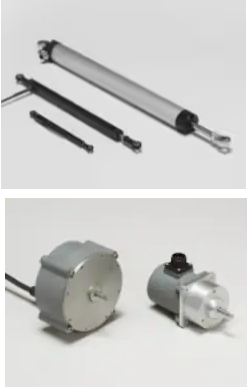
\includegraphics[width=0.3\linewidth]{img/potenciometro}
		\caption{imagen de sensor}
		\label{fig:potenciometro}
	\end{figure}

\section{Imágenes}
En \LaTeX, las imágenes se pueden incluir utilizando el paquete \texttt{graphicx}. 
Para añadir una imagen en texstudio, es posible arrastrarla directamente en el editor, lo que obtendrá como resultado lo mostrado en la \autoref{fig:insertarimagen}.

\begin{figure}[h]
	\centering
	\includegraphics[width=0.7\linewidth]{img/insertarImagen}
	\caption{Opciones al insertar una imagen}
	\label{fig:insertarimagen}
\end{figure}

Algunas opciones clave incluyen:

\begin{itemize}
	\item \textbf{Tamaño de la imagen}: Se puede definir un ancho o alto relativo a la caja de texto o se puede usar un tamaño en pixeles (px), centímetros (cm) o el ancho de la letra M (em).
	\item \textbf{Centrado}: Se puede marcar la opción para que la imagen aparezca centrada automáticamente.
	\item \textbf{Uso del entorno `figure'}: Permite que la imagen tenga una numeración automática y pueda referenciarse en el texto con \texttt{\textbackslash ref\{\}} o \texttt{\textbackslash autoref\{\}}.
	\item \textbf{Posicionamiento (`h`, `t`, `b`, `p`)}: Al presionar la flecha de la derecha, podemos añadir las opciones que determinan la posición de la imagen en el documento, como después del texto o arriba de la página, etc. Si igual vamos a referenciar las figuras, es innecesario que estén exactamente donde fueron mencionadas ya que eso deja muchos espacios en blanco.
	\item \textbf{Leyenda Largo}: permite poner una descripción de la imagen en el lugar que elegimos (debería de estar debajo).
	\item \textbf{Etiqueta}: nos servirá para referenciarla. 
\end{itemize}

Para usar dos imágenes como en \autoref{fig:mascotas}, se utilizó \texttt{subfloat}.
% Dos imágenes de mascotas
\begin{figure}[h]
	\centering
	\subfloat[Perro]{%
		\includegraphics[width=0.4\textwidth]{perro.jpg}%
		\label{fig:perro}
	}
	\hfill
	\subfloat[Gato]{%
		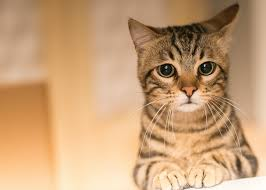
\includegraphics[width=0.4\textwidth]{gato.jpg}%
		\label{fig:gato}
	}
	\caption{Imagen de dos mascotas}
	\label{fig:mascotas}
\end{figure}
\\
\newpage
\section{SENSOR DE VELOCIDAD}
Dispositivo que mide la rapidez con la que un objeto se mueve. Puede basarse en principios ópticos, magnéticos o mecánicos para calcular la velocidad de giro o desplazamiento.
Sensor automotriz de velocidad y transmisión.\autoref{fig:sensor de velocidad}
\begin{figure}[h]
	\centering
	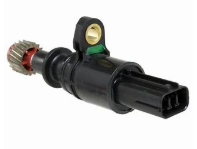
\includegraphics[width=0.3\linewidth]{img/sensor de velocidad}
	\caption{Sensor de velocidad}
	\label{fig:sensor de velocidad}
\end{figure}

\section*{TACOMETRO}
Sensor que mide la velocidad de rotación de un eje o motor, generalmente en revoluciones por minuto (RPM). Puede ser mecánico, óptico o basado en efecto Hall.

\section*{SENSOR DE EFECTO HALL}
Estos sensores detectan la velocidad midiendo cambios en el campo magnético generado por un imán o un objeto ferroso en movimiento. Son ampliamente utilizados en aplicaciones automotrices, como la medición de la velocidad de las ruedas en los sistemas de frenos antibloqueo, y para medir corriente eléctrica.

\begin{figure}[h]
	\centering
	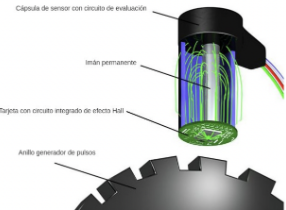
\includegraphics[width=0.3\linewidth]{img/HALL}
	\caption{Sensor de velocidad}
	\label{fig:HALL}
\end{figure}



\newpage
\section{FUERZA}
\section{GALGAS EXTENSIOMETRICAS}
Las galgas extensométricas son sensores que miden la deformación de un objeto. Su funcionamiento se basa en el efecto piezorresistivo, donde la resistencia eléctrica del material cambia al ser sometido a esfuerzos mecánicos. Cuando se aplica una fuerza externa, el objeto se deforma, y esta deformación provoca una variación en la resistencia de la galga, que puede medirse y correlacionarse con la magnitud de la fuerza aplicada. Estos sensores son fundamentales en la medición de fuerzas, presiones y tensiones en diversas aplicaciones de ingeniería.\autoref{fig:GAL}
\begin{figure}[h]
	\centering
	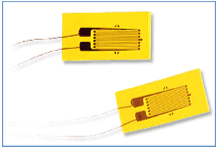
\includegraphics[width=0.3\linewidth]{img/GAL}
	\caption{Galgas }
	\label{fig:GAL}
\end{figure}

\section*{INTERRUPTOR DE EFECTO HALL}
Estos dispositivos detectan la presencia de un campo magnético. El efecto Hall se manifiesta cuando una corriente eléctrica que fluye a través de un semiconductor se ve afectada por un campo magnético perpendicular, generando una diferencia de potencial (voltaje Hall) transversal al flujo de corriente. Los interruptores de efecto Hall utilizan este principio para detectar campos magnéticos y, en consecuencia, activar o desactivar circuitos electrónicos. Son ampliamente utilizados en aplicaciones donde se requiere una detección precisa y sin contacto de posiciones o movimientos, como en sistemas de control de motores y dispositivos de seguridad.\autoref{fig:INTERRUPTOR HALL}
\begin{figure}[h]
	\centering
	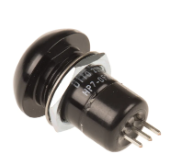
\includegraphics[width=0.3\linewidth]{img/INTERRUPTOR HALL}
	\caption{ Interruptor HALL }
	\label{fig:INTERRUPTOR HALL}
\end{figure}



\newpage
\section{INTERRUPTOR PIEZOELECTRICO }
Estos sensores\cite{TE_PiezoFilm} se basan en el efecto piezoeléctrico, donde ciertos materiales generan una carga eléctrica en respuesta a una deformación mecánica. Cuando se aplica una fuerza sobre un material piezoeléctrico, este se deforma y produce una tensión eléctrica proporcional a la magnitud de la fuerza aplicada. Los interruptores piezoeléctricos aprovechan este fenómeno para detectar cambios de presión o vibraciones, generando señales eléctricas que pueden utilizarse para activar o controlar otros dispositivos electrónicos. Son especialmente útiles en aplicaciones que requieren una respuesta rápida y alta sensibilidad, como en sensores táctiles y sistemas de monitoreo de vibraciones.
Estos sensores son fundamentales en aplicaciones de ingeniería electrónica y robótica, permitiendo la medición precisa de fuerzas y la detección de campos magnéticos, lo que es esencial para el control y monitoreo de sistemas mecánicos y electrónicos.\autoref{fig:PIEZO}
\begin{figure}[h]
	\centering
	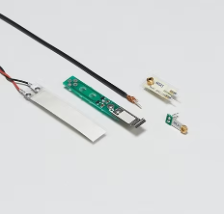
\includegraphics[width=0.3\linewidth]{img/PIEZO}
	\caption{Interruptor piezoecletrico  }
	\label{fig:PIEZO}
\end{figure}

\section{SENSORES EXTERNOS}
\section*{Tipo de contacto}
\section*{Interruptores de límite }
¿Qué es un sensor de contacto?
Los sensores de contacto\cite{Keyence_Contacto} son un tipo de sensor que detecta el final de recorrido de un componente mecánico, es decir, detecta la posición límite de este mismo.\cite{Cybermatics_Sensores} 
\begin{itemize}
	\item  Tipos de sensores de contacto.
	\item  Verticales 
	\item Horizontales 
	\item Micro
\end{itemize}

\begin{figure}[h]
	\centering
	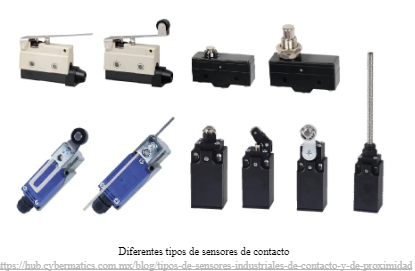
\includegraphics[width=0.3\linewidth]{img/CONTACTO}
	\caption{Sensores de contacto  }
	\label{fig:CONTACTO}
\end{figure}



\section{Funcionamiento de sensores de contacto } 
Dichos sensores poseen un switch que al entrar en contacto con una superficie, emite una señal eléctrica que activa o desactiva el paso de la energía. 
Al poseer una composición robusta,  es favorable para evitar choques al detener los actuadores. 

\section*{Ventajas}
\begin{itemize}
	\item Detección de objetos 
	\item  Prevención de choques  
	\item Automatización de procesos 
\end{itemize}


\section*{Aplicaciones de un sensor de contacto} 
\begin{itemize}
	\item Medición de fuerza y presión 
	\item Control de nivel líquido  
	\item Envío de señales de retorno 
	\item Control de posición de válvulas
\end{itemize}


\section{Giroscopio}
El giroscopio consiste en un sensor interno de posición que viene integrado en los dispositivos. Este permite al dispositivo conocer su orientación y posición en el espacio mediante tres sistemas integrados en el chip, cada uno jugando un rol en el eje “x”, “y” y “z” respectivamente.

En la imagen\autoref{fig:GIROSCOPIO} se puede observar 6 diferentes secciones del microchip. Las 3 partes superiores forman parte de un acelerómetro, mientras que las 3 partes inferiores son los tres sensores del giroscopio. Orientados de izquierda a derecha serían eje “z”, “x” y “x”.

\begin{figure}[h]
	\centering
	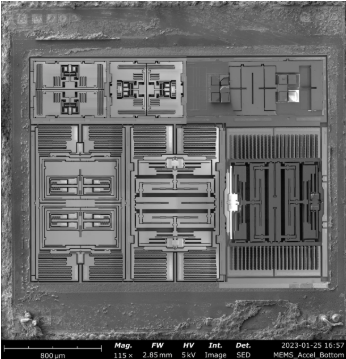
\includegraphics[width=0.3\linewidth]{img/GIROSCOPIO}
	\caption{Imagen de un Giroscopio  }
	\label{fig:GIROSCOPIO}
\end{figure}

Las partes de dirección  “x” y dirección “y” son básicamente la misma pieza pero rotada 90 grados. La parte direccional de “z” tiene una composición distinta a la de sus otras contrapartes.

El funcionamiento general del sistema utiliza un fenómeno conocido como efecto coriolis y algo parecido a la resonancia de un diapasón, ya que en conjunto de las fuerzas generadas por las vibraciones, las cuales hacen que dos piezas paralelas resuenen entre sí, más el efecto coriolis en la rotación, generando así una desviación en la frecuencia.



\newpage
 La imagen\autoref{fig:FLECHAS} se puede observar los dos elementos y la fuerza resultante de la desviación generada por la rotación. Las fuerzas F son generadas por la resonancia de las piezas en el sistema, las cuales mientras en una parte generan un movimiento resonante de tipo resorte, en la parte central generan un movimiento oscilatorio a una frecuencia previamente programada. Al momento de estar presente la rotación, se genera una desviación en las fuerzas, señalada en la imagen como S \cite{SICK_Encodersd}. Esto a su vez genera una desviación en las oscilaciones de la parte central de la pieza, lo cual provoca una diferencia en la frecuencia previamente programada, siendo esta diferencia detectada por una zona dentada del mecanismo.

El cambio de frecuencia se consideraría en este caso como cambio de posición en el espacio. 

Este proceso funciona de la misma manera en los tres ejes, dando así la capacidad a los dispositivos de saber en qué posición se encuentran dentro del espacio.
\begin{figure}[h]
	\centering
	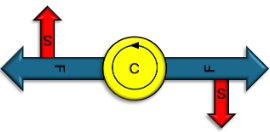
\includegraphics[width=0.3\linewidth]{img/FLECHAS}
	\caption{Direccion de fuerzas  }
	\label{fig:FLECHAS}
\end{figure}

\section{ACELEROMETRO}

Los acelerómetros\autoref{fig:ACE},se utilizan en mediciones de aceleración gravitacional estática como se aprecia en \cite{TME_Acelerometro}, lo que le permite determinar el ángulo de desviación del objeto medido de la vertical, así como en mediciones de aceleración dinámica debido a golpes, movimiento, impacto o vibración, es decir, vibraciones de baja amplitud y baja frecuencia, que alcanzan varias docenas de Hz.
\begin{figure}[h]
	\centering
	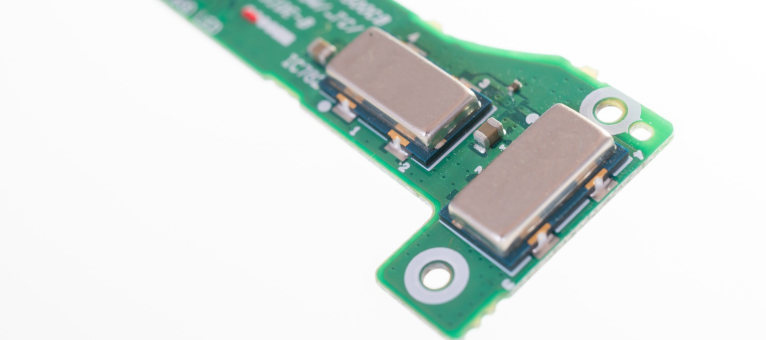
\includegraphics[width=0.3\linewidth]{img/ACE}
	\caption{Acelerometro }
	\label{fig:ACE}
\end{figure}


¿Cómo funciona un acelerómetro mientras se mide la vibración? Este dispositivo se implementa directamente en el objeto que vibra, lo que le permite convertir la energía de vibración en una señal eléctrica que es proporcional a la aceleración momentánea del objeto.

¿Qué hace un acelerómetro? La medición de la vibración se usa generalmente para diagnosticar el funcionamiento de máquinas, dispositivos o estructuras sometidas a altos esfuerzos, por ejemplo, estructuras de acero de mástiles, puentes o estructuras de edificios. También se utilizan acelerómetros, entre otros. para proteger los discos duros contra daños, en equipos médicos y deportivos, en cámaras y videocámaras, en teléfonos inteligentes, controles remotos, controladores o en sistemas de navegación.

¿Qué es un acelerómetro? No es más que un transductor de aceleración que mide su propio movimiento en el espacio. Hay tres tipos básicos de acelerómetros, más de los cuales más adelante en el artículo.


\newpage
	\section{MAGNETOMETRO}
	Un magnetómetro\autoref{fig:MAG} es un dispositivo capaz de identificar la dirección de referencia, normalmente el norte, a partir de la medición del campo magnético de la tierra.
	Existen\cite{ScienceDirect_Magnetometer} diferentes tipos de magnetómetros, el más sencillo es la brújula magnética, la cual rastrea la orientación de una aguja metálica dentro del campo magnético de la tierra.como se puede arpeciar en \cite{TransducerResearch_Magnetoresistive} Esta tiene ciertos problemas, como el que el norte magnético de la tierra no se alinea con el norte geográfico, necesitando entonces calibrar según la ubicación para considerar este desfase. Otro problema es que son fácilmente influenciadas por otras fuentes de campos magnéticos. 
		\begin{figure}[h]
		\centering
		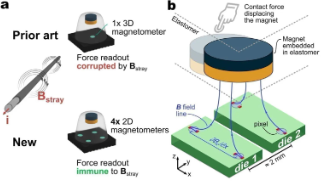
\includegraphics[width=0.3\linewidth]{img/MAG}
		\caption{Magnetometro }
		\label{fig:MAG}
	\end{figure}
	
	Las brújulas electrónicas pueden encontrar el norte magnético a partir de propiedades electrónicas. Estas normalmente utilizan el efecto Hall para su medición, aunque algunas utilizan el efecto magneto-resistivo.

	El efecto Hall se basa en las propiedades electromagnéticas de ciertos materiales, por ejemplo, si suministramos corriente a través de una placa metálica la cual a continuación se le aplica un campo magnético, dentro de la placa se distorsionara su campo eléctrico, por lo que un lado de la placa se cargará negativamente y el otro positivamente. Midiendo con un voltímetro las cargas de la placa podemos determinar que tan fuerte es el campo magnético.
	El efecto magneto-resistivo basa su funcionamiento en el hecho que ciertos materiales pueden cambiar su resistividad si son expuestos a un campo magnético.
	
	\section{LiDAR}
El LiDAR\autoref{fig:LiDAR} es un sensor que utiliza láseres para medir distancias, movimientos de un entorno, calcular superficies y mapear un espacio señalado \cite{IBM_Lidar}.
\begin{figure}[h]
	\centering
	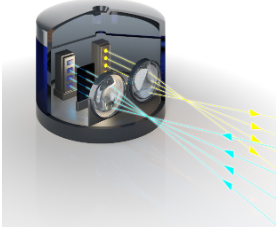
\includegraphics[width=0.3\linewidth]{img/LiDAR}
	\caption{Magnetometro }
	\label{fig:LiDAR}
\end{figure}

\section*{Tipos de sensores LiDAR:}
\begin{itemize}
	\item Topográfico 
	\item Batimétrico  
\end{itemize}





\section*{¿Cómo funciona un sensor LiDAR?}

\subsection*{Tipo Topográfico:}
El sensorautoref\autoref{fig:TOP} posee un escáner que emite rayos infrarrojos que rebotan en las superficies con las que impactan, posteriormente los rayos que vuelven al sensor son registrados por un receptor y se realiza una medición en función del tiempo y la velocidad de la luz. El sensor LiDAR dispara miles de rayos por segundo los cuales generan la llamada nube de puntos, estos al combinarse con información posicional GPS/INS, genera un mapeo de puntos tridimensionales en tiempo real.\cite{NOAA_Lidar} 
\begin{figure}[h]
	\centering
	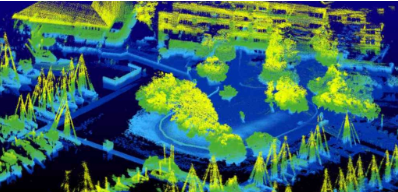
\includegraphics[width=0.3\linewidth]{img/TOP}
	\caption{Mapa topografico terrestre }
	\label{fig:TOP}
\end{figure}
\subsection*{Tipo Batimétrico:}
El sensor\autoref{fig:BAT} utiliza un escáner que emite luz verde, el cual es capaz de penetrar en el agua para hacer un mapeo completo de las profundidades costeras, lagos, ríos, etc. Con este tipo de escáner es posible detectar profundidades de hasta 10 metros.\cite{UAVLatam_Lidar}
\begin{figure}[h]
	\centering
	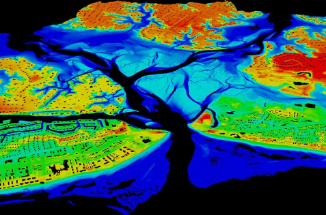
\includegraphics[width=0.3\linewidth]{img/BAT}
	\caption{Mapa de Lynnhavent,Virginia }
	\label{fig:BAT}
\end{figure}

Dicho escaneo puede tomar distintas formas:
\begin{itemize}
	\item Líneas: se producen líneas paralelas al momento de realizar el escaneado debido a que el sensor posee un espejo rotatorio que desvía el haz láser. 
	\item Zigzag: el espejo rotatorio produce líneas en forma de zigzag como patrón de escaneado debido a que el espejo es rotatorio en dos sentidos, ida y vuelta.  
	\item Fibra óptica: el haz láser es desviado desde un cable de fibra óptica, y el patrón de escaneado toma la forma de pequeñas circunferencias
	\item Elíptica: el patrón de escaneado toma forma elíptica, el cual se produce a través del desvío del haz láser por intermedio de dos espejos.
\end{itemize}

\subsection*{Componentes de un sensor LiDAR:}
\begin{itemize}
	\item Un escáner láser que emite pulsos rápidos de luz láser casi infrarroja
	\item Un sensor LiDAR utilizado para detectar y recoger los pulsos luminosos reflejados 
	\item Un procesador para calcular el tiempo y la distancia, así como para construir el conjunto de datos resultante, denominado nube de puntos LiDAR. 
\end{itemize}






%-------------------------------------------
% Bibliografía
%-------------------------------------------
\bibliographystyle{IEEEtran}  % Estilo de bibliografía IEEE
% La bibliografía se tomará del archivo "fuentes.bib"
%\newpage
\bibliography{fuentes}
	
\end{document}
